\section{Key characteristics}

\begin{frame}
\frametitle{Build on top of other open source image processing software}
\begin{block}{Motivations}
\begin{itemize}
\item Interfaces seamlessly with other image processing and remote sensing open-source software
\item Increase the number of functions
\item Combine tools to create hybrid data pipeline
\end{itemize}
\end{block}

\begin{block}{OTB backbone}
\begin{itemize}
\item \href{www.itk.org}{ITK}: data processing pipeline
\item \href{www.gdal.org}{GDAL}: read and write raster and vector data
\item \href{www.ossim.org}{OSSIM}: sensor modelling and metadata support
\item \href{www.opencv.org}{OpenCV} and \href{www.libsvm.org}{LibSVM}: machine learning algorithms
\item \href{www.muparser.org}{MuParser} and \href{www.muparserx.org}{MuParserX}:
  powerful parsing of mathematical expression (band math)
\end{itemize}
\end{block}

\end{frame}

\begin{frame}
\frametitle{Compatible (and available) on multiple platforms}
\begin{columns}
\column{0.5\textwidth}
\begin{block}{Goal}
\begin{itemize}
\item Compile with recent versions of:
\begin{itemize}
\item GCC
\item Clang
\item MinGW
\item Visual Studio\ldots
\end{itemize}
\item Binary packages available:
\begin{itemize}
\item UbuntuGIS repository (GIS and IP software for Ubuntu)
\item Experimental Debian packages
\item Available in  OSGeo4W (OSGeo tools on Windows)
\item Binary installers, Port and Brew formula for Mac OS X\ldots
\end{itemize}
\end{itemize}
\end{block}
\column{0.5\textwidth}
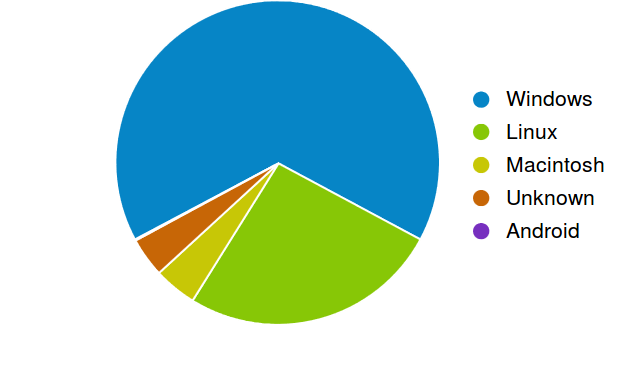
\includegraphics[width=\textwidth]{images/OTB4_download_sourceforge_os_crop.png}
\begin{center}
\tiny{Number of OTB downloads on Sourceforge per Operating System}
\end{center}
\end{columns}
\end{frame}

\begin{frame}
\frametitle{Flexibility, scalability: \textit{Pipeline}, \textit{Streaming} and \textit{multithreading}}

\begin{block}{\textit{Pipeline} data model}
\begin{center}
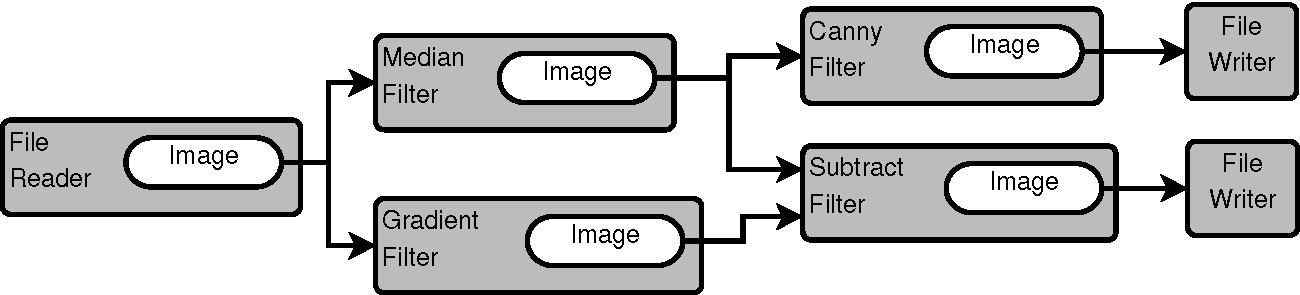
\includegraphics[width=0.7\textwidth]{images/ProcessObjectDataObject.png}
\end{center}
\end{block}
\vspace{-0.5cm}
\begin{block}{\textit{Streaming}}
\begin{center}
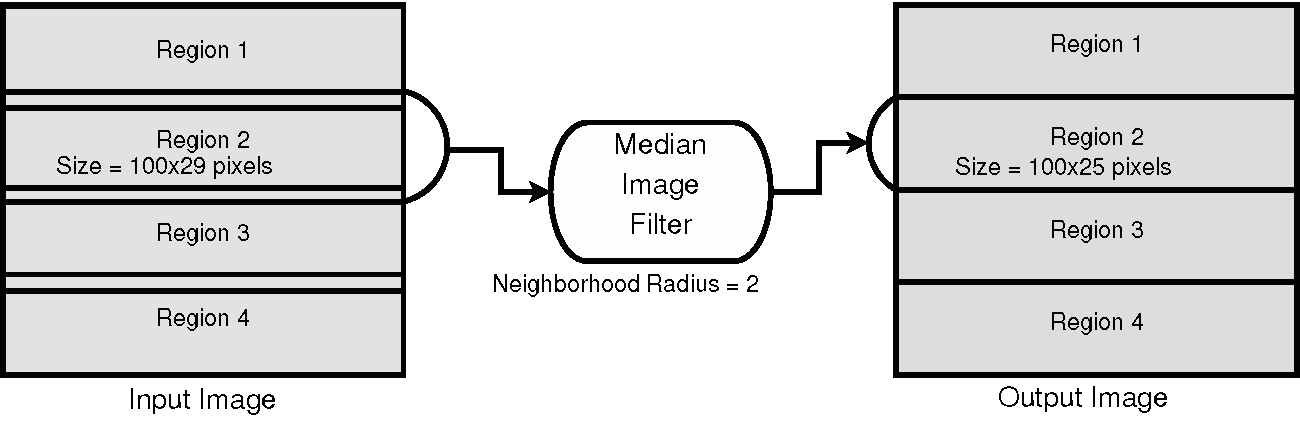
\includegraphics[width=0.7\textwidth]{images/StreamingImageDiagram.png}
\end{center}
\end{block}
\vspace{-0.5cm}
\begin{center}
\tiny{source: \url{http://www.aosabook.org/en/itk.html}}
\end{center}
\end{frame}

\begin{frame}
\frametitle{Behind the scene}
\begin{center}
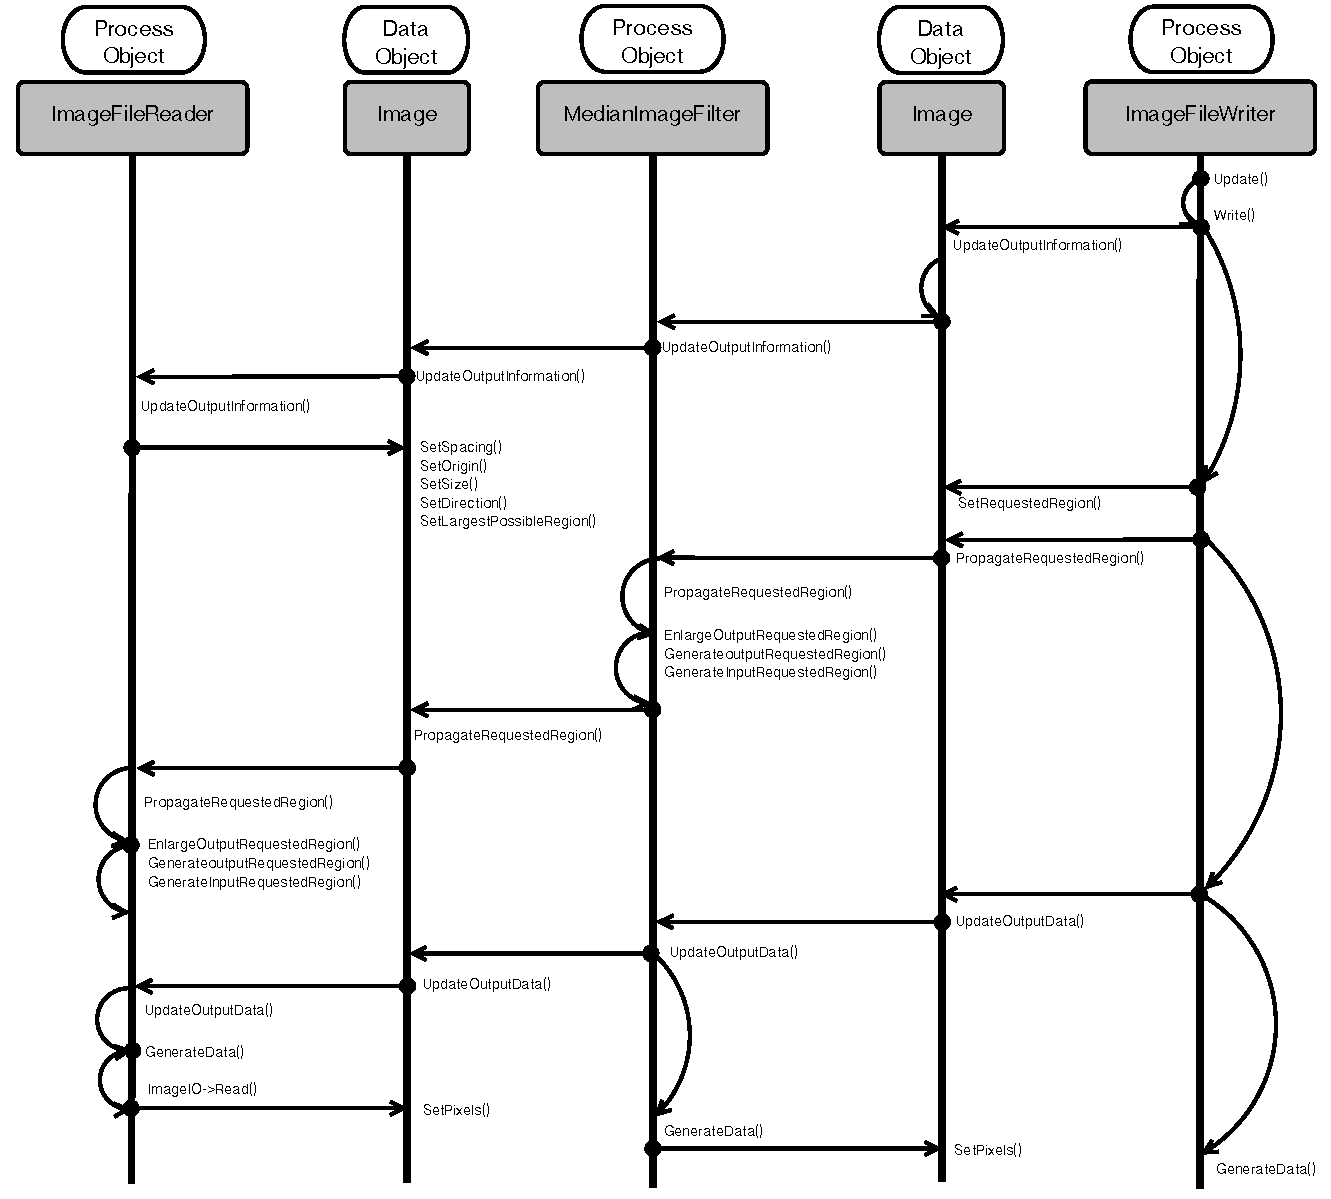
\includegraphics[width=0.7\textwidth]{images/ProcessObjectDataObjectInteractionUML.png}\\
\tiny{source: \url{http://www.aosabook.org/en/itk.html}}
\end{center}
\end{frame}

\begin{frame}
\frametitle{State of the art}
\begin{itemize}
\item Try to keep track of up-to-date information about the latest developments, exchanging ideas, identifying future trends, and making networking
\item Reference implementation of algorithms based on publications
\item e.g.: morphological profile, MeanShift segmentation, Haralick textures, SURF keypoints\ldots
\item Reference implementation contributes by authors with their
  publications. e.g.: Large Scale MeanShift, object detection \ldots
\end{itemize}
\end{frame}

\begin{frame}
\frametitle{How is OTB developed?}
\vspace{-0.5cm}
\begin{itemize}
\item Distributed version control: Git (migration from Mercurial in July 2015)
\item C++ and CMake (CTest, CDash)
\item Test driven development (TDD)
\item Agile (scrum)
\item Continuous integration and packaging
\end{itemize}
Every day, almost 3000 tests are compiled, launched on 16 different
configurations.
\begin{center}
\href{http://dash.orfeo-toolbox.org/index.php?project=OTB}{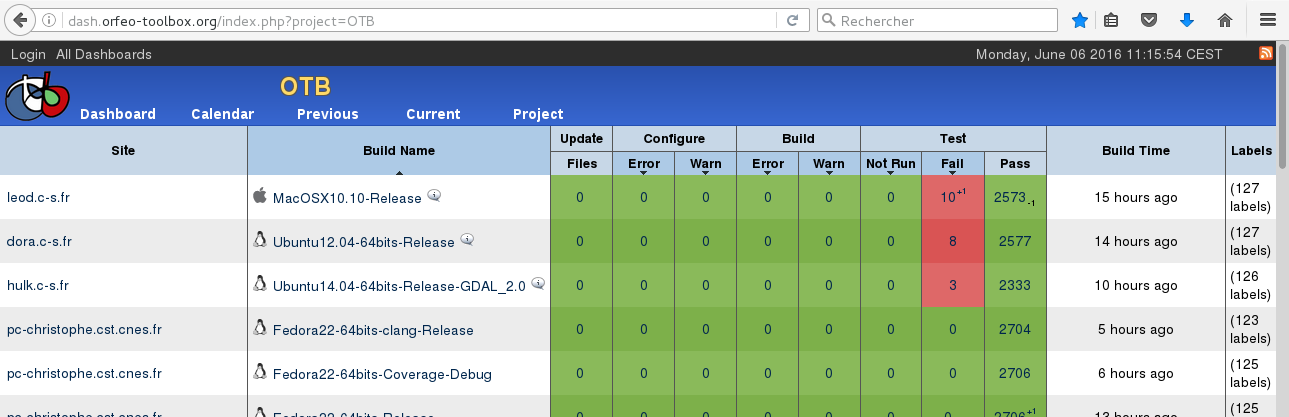
\includegraphics[width=\textwidth]{images/dashboard.png}}
\end{center}
\end{frame}
